\documentclass[12pt,a4paper]{article}
% Shared preamble for both books. Compile from the repository root.
\usepackage[margin=1in]{geometry}
\usepackage{amsmath,amssymb,amsfonts}
\usepackage{lmodern}
\usepackage{graphicx}
\usepackage{enumitem}
\usepackage{xcolor}
\usepackage[most]{tcolorbox}
% xr-hyper must precede hyperref so external labels carry PDF destinations.
\usepackage{xr-hyper}
\usepackage[hidelinks]{hyperref}
\hypersetup{linktoc=all}
\usepackage{fancyhdr}
\usepackage{microtype}
\usepackage{needspace}
\usepackage{xparse}
\usepackage{xstring}
\usepackage{caption}
\usepackage{siunitx}
\usepackage{etoolbox}
\usepackage{tikz}
\usetikzlibrary{arrows.meta}
\setlength{\headheight}{14.5pt}
\setlength{\emergencystretch}{2em}
\raggedbottom

\newcommand{\bookheader}{Physics Bowl}
\pagestyle{fancy}
\fancyhf{}
\fancyhead[L]{Ray Zhou}
\fancyhead[R]{\bookheader}
\fancyfoot[C]{\thepage}
\renewcommand{\headrulewidth}{0.4pt}
\fancypagestyle{plain}{%
  \fancyhf{}
  \fancyfoot[C]{\thepage}
  \renewcommand{\headrulewidth}{0pt}
}

\colorlet{ThemeFrame}{black!20}
\colorlet{ThemeTitle}{gray!15}
\newcommand{\setcheattheme}[2]{\colorlet{ThemeFrame}{#1}\colorlet{ThemeTitle}{#2}}
\newcommand{\parttheme}[1]{%
  \IfStrEqCase{#1}{%
    {mech}{\setcheattheme{teal!30}{teal!12}}%
    {waves}{\setcheattheme{yellow!35}{yellow!12}}%
    {em}{\setcheattheme{magenta!30}{magenta!12}}%
    {optics}{\setcheattheme{cyan!35}{cyan!12}}%
  }[\setcheattheme{black!20}{gray!15}]}
\tcbset{colback=white, boxrule=0.5pt, coltitle=black}
\newtcolorbox{formulabox}{enhanced, breakable, colframe=ThemeFrame,
  colbacktitle=ThemeTitle, title=\textbf{Concepts and Formulas},
  fonttitle=\bfseries, left=10pt, right=10pt, top=7pt, bottom=8pt,
  before skip=8pt, after skip=8pt}
\newtcolorbox{heuristicsbox}{enhanced, breakable, colframe=ThemeFrame,
  colbacktitle=ThemeTitle, title=\textbf{Methods and Pitfalls},
  fonttitle=\bfseries, left=10pt, right=10pt, top=7pt, bottom=8pt,
  before skip=8pt, after skip=8pt}
\newtcolorbox{solutionbox}{enhanced, breakable, colframe=black!25,
  colbacktitle=gray!12, title=\textbf{Solution}, fonttitle=\bfseries,
  left=10pt, right=10pt, top=7pt, bottom=8pt, before skip=6pt, after skip=8pt}
\newtcolorbox{insightbox}{enhanced, breakable, colback=blue!2,
  colframe=blue!35, colbacktitle=blue!12, title=\textbf{Key Insight},
  fonttitle=\bfseries, left=8pt, right=8pt, top=5pt, bottom=6pt,
  before skip=6pt, after skip=6pt}
\newtcolorbox{answerbox}{colback=white, colframe=white, boxrule=0pt,
  left=0pt, right=0pt, top=0pt, bottom=0pt, boxsep=0pt,
  before skip=2pt, after skip=4pt}
\newtcolorbox{disclaimerbox}{enhanced, breakable, colback=gray!6,
  colframe=gray!45, left=10pt, right=10pt, top=7pt, bottom=7pt,
  before skip=6pt, after skip=8pt, fontupper=\small}
\newcommand{\finalanswer}[1]{\textbf{Answer:}~#1}

% Internal learning labels; these are not official competition divisions.
\newcommand{\Core}{\texorpdfstring{\textsuperscript{\textbf{Core}}}{ [Core]}}
\newcommand{\Extension}{\texorpdfstring{\textsuperscript{\textbf{Extension}}}{ [Extension]}}

\graphicspath{{problems/figures/}}
\renewcommand{\bookheader}{Physics Bowl Selected Problems}
\externaldocument[g-]{CheatSheets}[CheatSheets.pdf]
% Generated by scripts/generate_crossrefs.py; edit data/problem-topics.json.
\newcommand{\SelectedProblem}[1]{\hyperref[p-prob:#1]{Problem~#1} (p.~\pageref{p-prob:#1})}
\newcommand{\GuideUnit}[2]{\hyperref[g-unit:#1]{#2}}
\newcommand{\UnitProblemLinks}[1]{\par\smallskip\noindent\textbf{Related problems:} \csname problem-links-#1\endcsname\par}
\newcommand{\StudyGuideLinks}[1]{\par\smallskip\noindent\textit{Study guide:} \csname guide-links-#1\endcsname\par}
\newcommand{\LocalProblem}[1]{\hyperref[prob:#1]{#1}}
\newcommand{\ProblemSource}[1]{\par\noindent{\footnotesize \textit{Source:} \csname source-#1\endcsname}\par}
\expandafter\def\csname problem-links-kinematics\endcsname{\SelectedProblem{1}, \SelectedProblem{10}, \SelectedProblem{13}, \SelectedProblem{18}, \SelectedProblem{26}, \SelectedProblem{27}, \SelectedProblem{30}, \SelectedProblem{35}, \SelectedProblem{39}}
\expandafter\def\csname problem-links-dynamics\endcsname{\SelectedProblem{2}, \SelectedProblem{5}, \SelectedProblem{14}, \SelectedProblem{16}, \SelectedProblem{23}, \SelectedProblem{27}, \SelectedProblem{28}, \SelectedProblem{36}}
\expandafter\def\csname problem-links-energy\endcsname{\SelectedProblem{2}, \SelectedProblem{14}, \SelectedProblem{17}, \SelectedProblem{20}, \SelectedProblem{28}}
\expandafter\def\csname problem-links-momentum\endcsname{\SelectedProblem{1}, \SelectedProblem{29}, \SelectedProblem{33}}
\expandafter\def\csname problem-links-rotation\endcsname{\SelectedProblem{15}, \SelectedProblem{16}, \SelectedProblem{20}, \SelectedProblem{38}}
\expandafter\def\csname problem-links-waves\endcsname{\SelectedProblem{3}, \SelectedProblem{24}, \SelectedProblem{31}}
\expandafter\def\csname problem-links-fluids-thermo\endcsname{\SelectedProblem{4}, \SelectedProblem{6}, \SelectedProblem{11}, \SelectedProblem{18}, \SelectedProblem{19}, \SelectedProblem{37}}
\expandafter\def\csname problem-links-electrostatics\endcsname{No selected problems in this unit yet.}
\expandafter\def\csname problem-links-circuits\endcsname{\SelectedProblem{7}, \SelectedProblem{9}, \SelectedProblem{12}, \SelectedProblem{22}}
\expandafter\def\csname problem-links-magnetism\endcsname{\SelectedProblem{8}}
\expandafter\def\csname problem-links-optics\endcsname{\SelectedProblem{21}, \SelectedProblem{25}, \SelectedProblem{34}}
\expandafter\def\csname problem-links-modern\endcsname{\SelectedProblem{32}}
\expandafter\def\csname guide-links-1\endcsname{\GuideUnit{kinematics}{Kinematics}; \GuideUnit{momentum}{Momentum and Collisions}}
\expandafter\def\csname source-1\endcsname{\href{https://www.aapt.org/programs/physicsbowl/upload/PhysicsBowl_2007.pdf}{AAPT PhysicsBowl 2007, problem 16 (PDF p.~4)}}
\expandafter\def\csname guide-links-2\endcsname{\GuideUnit{dynamics}{Newtonian Dynamics}; \GuideUnit{energy}{Work, Energy, Power}}
\expandafter\def\csname source-2\endcsname{\href{https://www.aapt.org/programs/physicsbowl/upload/PhysicsBowl_2007.pdf}{AAPT PhysicsBowl 2007, problem 22 (PDF p.~5)}}
\expandafter\def\csname guide-links-3\endcsname{\GuideUnit{waves}{Oscillations and Waves}}
\expandafter\def\csname source-3\endcsname{\href{https://www.aapt.org/programs/physicsbowl/upload/PhysicsBowl_2007.pdf}{AAPT PhysicsBowl 2007, problem 24 (PDF p.~6)}}
\expandafter\def\csname guide-links-4\endcsname{\GuideUnit{fluids-thermo}{Fluids and Thermodynamics}}
\expandafter\def\csname source-4\endcsname{\href{https://www.aapt.org/programs/physicsbowl/upload/PhysicsBowl_2007.pdf}{AAPT PhysicsBowl 2007, problem 39 (PDF p.~10)}}
\expandafter\def\csname guide-links-5\endcsname{\GuideUnit{dynamics}{Newtonian Dynamics}}
\expandafter\def\csname source-5\endcsname{\href{https://www.aapt.org/Programs/PhysicsBowl/upload/PhysicsBowl_2008_Exam.pdf}{AAPT PhysicsBowl 2008, problem 13 (PDF p.~3)}}
\expandafter\def\csname guide-links-6\endcsname{\GuideUnit{fluids-thermo}{Fluids and Thermodynamics}}
\expandafter\def\csname source-6\endcsname{\href{https://www.aapt.org/Programs/PhysicsBowl/upload/PhysicsBowl_2008_Exam.pdf}{AAPT PhysicsBowl 2008, problem 22 (PDF p.~4)}}
\expandafter\def\csname guide-links-7\endcsname{\GuideUnit{circuits}{DC Circuits}}
\expandafter\def\csname source-7\endcsname{\href{https://www.aapt.org/Programs/PhysicsBowl/upload/PhysicsBowl_2008_Exam.pdf}{AAPT PhysicsBowl 2008, problem 31 (PDF p.~6)}}
\expandafter\def\csname guide-links-8\endcsname{\GuideUnit{magnetism}{Magnetism and Induction}}
\expandafter\def\csname source-8\endcsname{\href{https://www.aapt.org/Programs/PhysicsBowl/upload/PhysicsBowl_2008_Exam.pdf}{AAPT PhysicsBowl 2008, problem 36 (PDF p.~7)}}
\expandafter\def\csname guide-links-9\endcsname{\GuideUnit{circuits}{DC Circuits}}
\expandafter\def\csname source-9\endcsname{\href{https://www.aapt.org/Programs/PhysicsBowl/upload/PhysicsBowl_2009_Exam.pdf}{AAPT PhysicsBowl 2009, problem 26 (PDF p.~5)}}
\expandafter\def\csname guide-links-10\endcsname{\GuideUnit{kinematics}{Kinematics}}
\expandafter\def\csname source-10\endcsname{\href{https://www.aapt.org/Programs/PhysicsBowl/upload/PhysicsBowl_2009_Exam.pdf}{AAPT PhysicsBowl 2009, problem 31 (PDF p.~6)}}
\expandafter\def\csname guide-links-11\endcsname{\GuideUnit{fluids-thermo}{Fluids and Thermodynamics}}
\expandafter\def\csname source-11\endcsname{\href{https://www.aapt.org/Programs/PhysicsBowl/upload/PhysicsBowl_2009_Exam.pdf}{AAPT PhysicsBowl 2009, problem 35 (PDF p.~7)}}
\expandafter\def\csname guide-links-12\endcsname{\GuideUnit{circuits}{DC Circuits}}
\expandafter\def\csname source-12\endcsname{\href{https://www.aapt.org/Programs/PhysicsBowl/upload/PhysicsBowl_2009_Exam.pdf}{AAPT PhysicsBowl 2009, problem 36 (PDF p.~7)}}
\expandafter\def\csname guide-links-13\endcsname{\GuideUnit{kinematics}{Kinematics}}
\expandafter\def\csname source-13\endcsname{\href{https://www.aapt.org/programs/physicsbowl/upload/PhysicsBowl_2010.pdf}{AAPT PhysicsBowl 2010, problem 29 (PDF p.~7)}}
\expandafter\def\csname guide-links-14\endcsname{\GuideUnit{dynamics}{Newtonian Dynamics}; \GuideUnit{energy}{Work, Energy, Power}}
\expandafter\def\csname source-14\endcsname{\href{https://www.aapt.org/programs/physicsbowl/upload/PhysicsBowl_2010.pdf}{AAPT PhysicsBowl 2010, problem 31 (PDF p.~7)}}
\expandafter\def\csname guide-links-15\endcsname{\GuideUnit{rotation}{Rotational Motion}}
\expandafter\def\csname source-15\endcsname{\href{https://www.aapt.org/programs/physicsbowl/upload/PhysicsBowl_2010.pdf}{AAPT PhysicsBowl 2010, problem 35 (PDF p.~8)}}
\expandafter\def\csname guide-links-16\endcsname{\GuideUnit{dynamics}{Newtonian Dynamics}; \GuideUnit{rotation}{Rotational Motion}}
\expandafter\def\csname source-16\endcsname{\href{https://www.aapt.org/programs/physicsbowl/upload/PhysicsBowl_2010.pdf}{AAPT PhysicsBowl 2010, problem 40 (PDF p.~9)}}
\expandafter\def\csname guide-links-17\endcsname{\GuideUnit{energy}{Work, Energy, Power}}
\expandafter\def\csname source-17\endcsname{\href{https://www.aapt.org/programs/physicsbowl/upload/PhysicsBowl_2010.pdf}{AAPT PhysicsBowl 2010, problem 42 (PDF p.~10)}}
\expandafter\def\csname guide-links-18\endcsname{\GuideUnit{kinematics}{Kinematics}; \GuideUnit{fluids-thermo}{Fluids and Thermodynamics}}
\expandafter\def\csname source-18\endcsname{\href{https://www.aapt.org/programs/physicsbowl/upload/PhysicsBowl_2010.pdf}{AAPT PhysicsBowl 2010, problem 47 (PDF p.~11)}}
\expandafter\def\csname guide-links-19\endcsname{\GuideUnit{fluids-thermo}{Fluids and Thermodynamics}}
\expandafter\def\csname source-19\endcsname{\href{https://www.aapt.org/programs/physicsbowl/upload/PhysicsBowl_2010.pdf}{AAPT PhysicsBowl 2010, problem 49 (PDF p.~11)}}
\expandafter\def\csname guide-links-20\endcsname{\GuideUnit{energy}{Work, Energy, Power}; \GuideUnit{rotation}{Rotational Motion}}
\expandafter\def\csname source-20\endcsname{\href{https://www.aapt.org/programs/physicsbowl/upload/PhysicsBowl_2012.pdf}{AAPT PhysicsBowl 2012, problem 33 (PDF p.~8)}}
\expandafter\def\csname guide-links-21\endcsname{\GuideUnit{optics}{Optics}}
\expandafter\def\csname source-21\endcsname{\href{https://www.aapt.org/programs/physicsbowl/upload/PhysicsBowl_2012.pdf}{AAPT PhysicsBowl 2012, problem 35 (PDF p.~8)}}
\expandafter\def\csname guide-links-22\endcsname{\GuideUnit{circuits}{DC Circuits}}
\expandafter\def\csname source-22\endcsname{\href{https://www.aapt.org/programs/physicsbowl/upload/PhysicsBowl_2012.pdf}{AAPT PhysicsBowl 2012, problem 39 (PDF p.~9)}}
\expandafter\def\csname guide-links-23\endcsname{\GuideUnit{dynamics}{Newtonian Dynamics}}
\expandafter\def\csname source-23\endcsname{\href{https://www.aapt.org/Programs/PhysicsBowl/upload/2015-PhysicsBowl-Final.pdf}{AAPT PhysicsBowl 2015, problem 24 (PDF p.~6)}}
\expandafter\def\csname guide-links-24\endcsname{\GuideUnit{waves}{Oscillations and Waves}}
\expandafter\def\csname source-24\endcsname{\href{https://www.aapt.org/Programs/PhysicsBowl/upload/2015-PhysicsBowl-Final.pdf}{AAPT PhysicsBowl 2015, problem 26 (PDF p.~7)}}
\expandafter\def\csname guide-links-25\endcsname{\GuideUnit{optics}{Optics}}
\expandafter\def\csname source-25\endcsname{\href{https://www.aapt.org/Programs/PhysicsBowl/upload/2015-PhysicsBowl-Final.pdf}{AAPT PhysicsBowl 2015, problem 34 (PDF p.~8)}}
\expandafter\def\csname guide-links-26\endcsname{\GuideUnit{kinematics}{Kinematics}}
\expandafter\def\csname source-26\endcsname{\href{https://www.aapt.org/Programs/PhysicsBowl/upload/2015-PhysicsBowl-Final.pdf}{AAPT PhysicsBowl 2015, problem 36 (PDF p.~9)}}
\expandafter\def\csname guide-links-27\endcsname{\GuideUnit{dynamics}{Newtonian Dynamics}; \GuideUnit{kinematics}{Kinematics}}
\expandafter\def\csname source-27\endcsname{\href{https://www.aapt.org/Programs/PhysicsBowl/upload/2015-PhysicsBowl-Final.pdf}{AAPT PhysicsBowl 2015, problem 40 (PDF p.~9)}}
\expandafter\def\csname guide-links-28\endcsname{\GuideUnit{dynamics}{Newtonian Dynamics}; \GuideUnit{energy}{Work, Energy, Power}}
\expandafter\def\csname source-28\endcsname{\href{https://www.aapt.org/Programs/PhysicsBowl/upload/PhysicsBowl_2017.pdf}{AAPT PhysicsBowl 2017, problem 25 (PDF p.~6)}}
\expandafter\def\csname guide-links-29\endcsname{\GuideUnit{momentum}{Momentum and Collisions}}
\expandafter\def\csname source-29\endcsname{\href{https://www.aapt.org/Programs/PhysicsBowl/upload/PhysicsBowl_2017.pdf}{AAPT PhysicsBowl 2017, problem 34 (PDF p.~8)}}
\expandafter\def\csname guide-links-30\endcsname{\GuideUnit{kinematics}{Kinematics}}
\expandafter\def\csname source-30\endcsname{\href{https://www.aapt.org/Programs/PhysicsBowl/upload/2018-PhysicsBowl-Exam-2.pdf}{AAPT PhysicsBowl 2018, problem 28 (PDF p.~5)}}
\expandafter\def\csname guide-links-31\endcsname{\GuideUnit{waves}{Oscillations and Waves}}
\expandafter\def\csname source-31\endcsname{\href{https://www.aapt.org/Programs/PhysicsBowl/upload/2018-PhysicsBowl-Exam-2.pdf}{AAPT PhysicsBowl 2018, problem 39 (PDF p.~6)}}
\expandafter\def\csname guide-links-32\endcsname{\GuideUnit{modern}{Modern Physics}}
\expandafter\def\csname source-32\endcsname{\href{https://www.aapt.org/Programs/PhysicsBowl/upload/2018-PhysicsBowl-Exam-2.pdf}{AAPT PhysicsBowl 2018, problem 49 (PDF p.~7)}}
\expandafter\def\csname guide-links-33\endcsname{\GuideUnit{momentum}{Momentum and Collisions}}
\expandafter\def\csname source-33\endcsname{\href{https://www.aapt.org/Programs/PhysicsBowl/upload/2019-PhysicsBowl-Exam.pdf}{AAPT PhysicsBowl 2019, problem 16 (PDF p.~5)}}
\expandafter\def\csname guide-links-34\endcsname{\GuideUnit{optics}{Optics}}
\expandafter\def\csname source-34\endcsname{\href{https://www.aapt.org/Programs/PhysicsBowl/upload/2019-PhysicsBowl-Exam.pdf}{AAPT PhysicsBowl 2019, problem 21 (PDF p.~5)}}
\expandafter\def\csname guide-links-35\endcsname{\GuideUnit{kinematics}{Kinematics}}
\expandafter\def\csname source-35\endcsname{\href{https://www.aapt.org/Programs/PhysicsBowl/upload/2019-PhysicsBowl-Exam.pdf}{AAPT PhysicsBowl 2019, problem 33 (PDF p.~7)}}
\expandafter\def\csname guide-links-36\endcsname{\GuideUnit{dynamics}{Newtonian Dynamics}}
\expandafter\def\csname source-36\endcsname{\href{https://www.aapt.org/Programs/PhysicsBowl/upload/2019-PhysicsBowl-Exam.pdf}{AAPT PhysicsBowl 2019, problem 43 (PDF p.~9)}}
\expandafter\def\csname guide-links-37\endcsname{\GuideUnit{fluids-thermo}{Fluids and Thermodynamics}}
\expandafter\def\csname source-37\endcsname{\href{https://www.aapt.org/Programs/PhysicsBowl/upload/2021-PhysicsBowl-Exam-2.pdf}{AAPT PhysicsBowl 2021, problem 16 (PDF p.~4)}}
\expandafter\def\csname guide-links-38\endcsname{\GuideUnit{rotation}{Rotational Motion}}
\expandafter\def\csname source-38\endcsname{\href{https://www.aapt.org/Programs/PhysicsBowl/upload/2021-PhysicsBowl-Exam-2.pdf}{AAPT PhysicsBowl 2021, problem 35 (PDF p.~8)}}
\expandafter\def\csname guide-links-39\endcsname{\GuideUnit{kinematics}{Kinematics}}
\expandafter\def\csname source-39\endcsname{\href{https://www.aapt.org/Programs/PhysicsBowl/upload/PhysicsBowl_2017.pdf}{AAPT PhysicsBowl 2017, problem 32 (PDF p.~7)}}
\newcommand{\ProblemTopicIndex}{%
\begin{itemize}[leftmargin=*]
\item \GuideUnit{kinematics}{Kinematics}: \LocalProblem{1}, \LocalProblem{10}, \LocalProblem{13}, \LocalProblem{18}, \LocalProblem{26}, \LocalProblem{27}, \LocalProblem{30}, \LocalProblem{35}, \LocalProblem{39}
\item \GuideUnit{dynamics}{Newtonian Dynamics}: \LocalProblem{2}, \LocalProblem{5}, \LocalProblem{14}, \LocalProblem{16}, \LocalProblem{23}, \LocalProblem{27}, \LocalProblem{28}, \LocalProblem{36}
\item \GuideUnit{energy}{Work, Energy, Power}: \LocalProblem{2}, \LocalProblem{14}, \LocalProblem{17}, \LocalProblem{20}, \LocalProblem{28}
\item \GuideUnit{momentum}{Momentum and Collisions}: \LocalProblem{1}, \LocalProblem{29}, \LocalProblem{33}
\item \GuideUnit{rotation}{Rotational Motion}: \LocalProblem{15}, \LocalProblem{16}, \LocalProblem{20}, \LocalProblem{38}
\item \GuideUnit{waves}{Oscillations and Waves}: \LocalProblem{3}, \LocalProblem{24}, \LocalProblem{31}
\item \GuideUnit{fluids-thermo}{Fluids and Thermodynamics}: \LocalProblem{4}, \LocalProblem{6}, \LocalProblem{11}, \LocalProblem{18}, \LocalProblem{19}, \LocalProblem{37}
\item \GuideUnit{electrostatics}{Electrostatics}: no selected problems
\item \GuideUnit{circuits}{DC Circuits}: \LocalProblem{7}, \LocalProblem{9}, \LocalProblem{12}, \LocalProblem{22}
\item \GuideUnit{magnetism}{Magnetism and Induction}: \LocalProblem{8}
\item \GuideUnit{optics}{Optics}: \LocalProblem{21}, \LocalProblem{25}, \LocalProblem{34}
\item \GuideUnit{modern}{Modern Physics}: \LocalProblem{32}
\end{itemize}}

\newcommand{\category}[1]{\par\smallskip\noindent\textit{Topic: #1}}
\newcommand{\categories}[1]{\category{#1}}

\begin{document}
\hypersetup{pageanchor=false}
\begin{titlepage}
\thispagestyle{empty}
\centering
\vspace*{2.2cm}
{\Huge\bfseries Physics Bowl Selected Problems\par}
\vspace{0.7cm}
{\Large 39 Problems, Key Insights, and Solutions\par}
\vspace{0.5cm}
{\large Companion to the Physics Bowl Study Guide\par}
\vfill
{\large Ray Zhou\par}
\end{titlepage}
\hypersetup{pageanchor=true}
\pagestyle{plain}
\pagenumbering{roman}
\section*{Using the Problem Set}
Work the question first, then compare your reasoning with the key insight and solution. Follow the study-guide links to review the underlying concepts.

The questions are adapted from AAPT PhysicsBowl past exams, with the source year, original question number and PDF page shown for each problem. Some figures are reproduced from those exams; the conical-pendulum diagram in problem 27 was redrawn. Consult the \href{https://www.aapt.org/Programs/PhysicsBowl/printexams.cfm}{official AAPT archive} for complete exams and solutions.
\subsection*{Notation and Conventions}
\begin{itemize}[leftmargin=*]
  \item Use SI units and $g=9.8\,\mathrm{m/s^2}$ unless a problem explicitly specifies another value. Angles are in radians unless degrees are shown.
  \item Arrows denote vectors, and $v=\lVert\vec v\rVert$ denotes a magnitude.
  \item $\mathcal E$ denotes electromotive force, while $\vec E$ denotes electric field. Circuit voltage is $V$.
  \item In thermodynamics $\Delta U=Q+W_{\rm on}$, where $W_{\rm on}>0$ is work done on the system. Equivalently, $\Delta U=Q-W_{\rm by}$.
  \item For thin lenses, the examples use real-object and real-image distances as positive. Check the chosen sign convention before substitution.
  \item Keep extra digits during calculations and round the final result consistently with the stated data.
\end{itemize}


\section*{Problem Index by Topic}
The numbers below link to problems in this document. Topic names link to the companion study guide.
\ProblemTopicIndex

\clearpage
\pagenumbering{arabic}
\pagestyle{fancy}
\begin{enumerate}[itemsep=1.2em, topsep=0.6em]
% Problem 1
\Needspace{18\baselineskip}
\item \label{prob:1}
Two identical mass objects are launched with the same speed from the same starting location. Object 1 is launched at an angle of $30^\circ$ above the horizontal while Object 2 is launched at an angle of $60^\circ$ above the horizontal. Ignore air resistance and consider the flight of each object from launch until it returns to the same launch height above the ground. Which object experiences the greatest change in the linear momentum?
\begin{enumerate}[label=(\Alph*)]
    \item Object 1 since it has a higher final speed.
    \item Object 2 since it has a higher final speed.
    \item Object 2 since it is in the air for a longer time.
    \item The change in momentum is the same for each.
    \item It cannot be determined without more information.
\end{enumerate}

\category{Kinematics \& Momentum}
\StudyGuideLinks{1}
\ProblemSource{1}
\begin{answerbox}
\finalanswer{(C) Object 2 since it is in the air for a longer time.}
\end{answerbox}
\begin{insightbox}
Impulse $J=\int F\,dt=mgT$ (only weight acts). For the same launch speed $v_0$, the time in the air is $T=\tfrac{2v_0\sin\theta}{g}$, so $|\Delta\vec p|=mgT=2mv_0\sin\theta$ increases with $\sin\theta$.
\end{insightbox}
\begin{solutionbox}
Gravity supplies impulse $\Delta\vec p=m\vec gT$. For a return to the launch height, $T=2v_0\sin\theta/g$, so
\[
 |\Delta\vec p|=mgT=2mv_0\sin\theta.
\]
Both objects have the same mass and launch speed, and $\sin60^\circ>\sin30^\circ$. Object 2 therefore has the greater momentum change.
\end{solutionbox}

% Problem 2
\Needspace{18\baselineskip}
\item \label{prob:2}
A mass $m$ is pulled outward until the string of length $L$ to which it is attached makes a 90-degree angle with the vertical. The mass is released from rest and swings through a circular arc. What is the tension in the string when the mass swings through the bottom of the arc?
\begin{enumerate}[label=(\Alph*)]
    \item 0
    \item $mg$
    \item $2mg$
    \item $3mg$
    \item It cannot be determined.
\end{enumerate}

\category{Circular Motion \& Energy}
\StudyGuideLinks{2}
\ProblemSource{2}
\begin{answerbox}
\finalanswer{(D) 3mg}
\end{answerbox}
\begin{insightbox}
Use energy to get $v^2=2gL$ at the bottom, then $T-mg=mv^2/L$.
\end{insightbox}
\begin{solutionbox}
By conservation of energy from the side to the bottom:
\begin{align*}
E_i &= K_i + U_i = 0 + mgL = mgL \\
E_f &= K_f + U_f = \tfrac{1}{2}mv^2 + 0
\end{align*}
Thus $mgL = \tfrac{1}{2}mv^2 \Rightarrow v^2 = 2gL$. At the bottom, radial (inward from the pivot) force balance yields
\[
T - mg = \frac{mv^2}{L} = \frac{m(2gL)}{L} = 2mg \Rightarrow T = 3mg.
\]
\\
\emph{Used:} conservation of mechanical energy and $F_c=mv^2/r$.
\end{solutionbox}

% Problem 3
\Needspace{18\baselineskip}
\item \label{prob:3}
\noindent\begin{minipage}[t]{0.6\linewidth}
\vspace{0pt} % Ensures top alignment
A resonance occurs with a tuning fork and an air column of size 39 cm. The next highest resonance occurs with an air column of 65 cm. What is the frequency of the tuning fork? Assume that the speed of sound is 343 m/s.
\begin{enumerate}[label=(\Alph*)]
    \item 329.8 Hz
    \item 527.7 Hz
    \item 659.6 Hz
    \item 879.5 Hz
    \item 1319 Hz
\end{enumerate}
\end{minipage}%
\hfill
\begin{minipage}[t]{0.33\linewidth}
\vspace{0pt} % Ensures top alignment
\centering
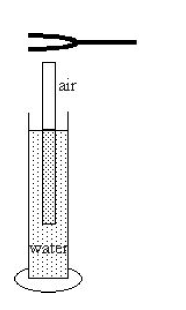
\includegraphics[width=0.7\linewidth]{Problem_03_Figure.png}
\end{minipage}

\category{Waves \& Sound}
\StudyGuideLinks{3}
\ProblemSource{3}
\begin{answerbox}
\finalanswer{(C) 659.6 Hz}
\end{answerbox}
\begin{insightbox}
Closed-tube resonances are spaced by $\lambda/2$; determine $\lambda$ from the difference in lengths and compute $f=v/\lambda$.
\end{insightbox}
\begin{solutionbox}

For a closed tube, successive resonances differ by $\Delta L = \tfrac{\lambda}{2}$. In this case $\Delta L = 0.65\,\text{m} - 0.39\,\text{m} = 0.26\,\text{m}$, so $\lambda = 2\times 0.26 = 0.52\,\text{m}$. The frequency is
\[
 f = \frac{v}{\lambda} = \frac{343\,\text{m/s}}{0.52\,\text{m}} \approx 659.6\,\text{Hz}.
\]
\\
\emph{Model:} closed–open tube has harmonics $L=(2n-1)\lambda/4$, so successive $L$ differ by $\lambda/2$.
\end{solutionbox}

% Problem 4
\Needspace{18\baselineskip}
\item \label{prob:4}
A mass of material exists in its solid form at its melting temperature $10^\circ$C. The following processes then occur to the material:
\begin{itemize}
    \item Process 1: An amount of thermal energy $Q$ is added to the material and $\tfrac{3}{4}$ of the material melts.
    \item Process 2: An identical additional amount of thermal energy $Q$ is added to the material and the material is now a liquid at $50^\circ$C.
\end{itemize}
What is the ratio of the latent heat of fusion to the specific heat of the liquid for this material?
\begin{enumerate}[label=(\Alph*)]
    \item $80^\circ$C
    \item $60^\circ$C
    \item $40^\circ$C
    \item $20^\circ$C
    \item More information is needed to answer this question.
\end{enumerate}

\category{Thermodynamics \& Phase Change}
\StudyGuideLinks{4}
\ProblemSource{4}
\begin{answerbox}
\finalanswer{(A) 80$^{\circ}$C}
\end{answerbox}
\begin{insightbox}
Two equal heat inputs: first melts 3/4, second completes melting 1/4 and warms; equate heats to find $L_f/c_l$.
\end{insightbox}
\begin{solutionbox}

Let mass $m$, latent heat $L_f$, liquid specific heat $c_l$, melting temperature $T_m=10^{\circ}\text{C}$. Process 1: $Q=\tfrac{3}{4}mL_f$. Process 2: $Q=\tfrac{1}{4}mL_f + mc_l(50-10)$. Equate:
\begin{align*}
\tfrac{3}{4} mL_f &= \tfrac{1}{4} mL_f + 40 m c_l \\
\tfrac{1}{2} mL_f &= 40 m c_l \Rightarrow \frac{L_f}{c_l} = 80\,\mathrm K.
\end{align*}
This is a temperature difference of $80^\circ\mathrm C$, corresponding to choice A.
\end{solutionbox}

% Problem 5
\Needspace{18\baselineskip}
\item \label{prob:5}
\noindent\begin{minipage}[t]{0.6\linewidth}
\vspace{0pt}
What is the ideal mechanical advantage for the pulley system shown in the figure?
\begin{enumerate}[label=(\Alph*)]
    \item $F/Mg$
    \item $Mg/F$
    \item 3
    \item 4
    \item 5
\end{enumerate}
\end{minipage}%
\hfill
\begin{minipage}[t]{0.33\linewidth}
\vspace{0pt}
\centering
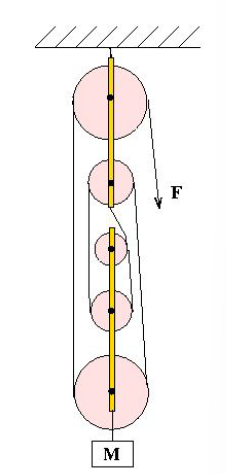
\includegraphics[width=0.6\linewidth]{Problem_05_Figure.png}
\end{minipage}

\category{Simple Machines \& Statics}
\StudyGuideLinks{5}
\ProblemSource{5}
\begin{answerbox}
\finalanswer{(D) 4}
\end{answerbox}
\begin{insightbox}
Ideal mechanical advantage equals the number of load-supporting rope segments: 4.
\end{insightbox}
\begin{solutionbox}

The ideal mechanical advantage equals the number of rope segments supporting the load. Here the movable block is supported by 4 segments, so $\text{IMA}=4$.
\\
\emph{Reminder:} massless, frictionless rope $\Rightarrow$ equal tension in all supporting segments.
\end{solutionbox}

% Problem 6
\Needspace{18\baselineskip}
\item \label{prob:6}
In a calorimeter, 20 grams of liquid water at $100^\circ$C is mixed with 50 grams of water vapor at $100^\circ$C. The system is allowed to come to equilibrium. Assume the phases coexist at their saturation pressure and the calorimeter and surroundings can be ignored. Which choice best describes the net energy exchange between the vapor and liquid?
\begin{enumerate}[label=(\Alph*)]
    \item There is no net energy exchange.
    \item Energy is transferred from the vapor to the liquid, vaporizing some of the liquid.
    \item Energy is transferred from the vapor to the liquid, increasing the liquid’s temperature.
    \item Energy is transferred from the vapor to the liquid until all of the liquid vaporizes.
    \item Energy is transferred from the vapor to the liquid, condensing some of the vapor.
\end{enumerate}

\category{Thermodynamics \& Phase Equilibrium}
\StudyGuideLinks{6}
\ProblemSource{6}
\begin{answerbox}
\finalanswer{(A) There is no net energy exchange.}
\end{answerbox}
\begin{insightbox}
At 100\textcelsius\ both phases are at the same temperature. In an isolated system the mixture stays at 100\textcelsius; any condensation of vapor must be balanced by vaporization of the same mass of liquid, so the net energy transferred between phases is zero.
\end{insightbox}
\begin{solutionbox}

As both steam and water are initially at the saturation temperature 100°C and the container is isolated (no heat to the surroundings), the final temperature is still 100°C. Let a mass $m_c$ of vapor condense (releasing $m_cL_v$) and a mass $m_v$ of liquid evaporate (absorbing $m_vL_v$). Conservation of energy for the constant-temperature closed system requires $m_cL_v=m_vL_v\Rightarrow m_c=m_v$. Therefore, the energy transferred from vapor to liquid equals the energy transferred from liquid to vapor, and the net energy transfer between the two phases is zero.
\end{solutionbox}

% Problem 7
\Needspace{18\baselineskip}
\item \label{prob:7}
\noindent\begin{minipage}[t]{0.6\linewidth}
\vspace{0pt}
For the circuit shown, $\varepsilon = 6.0$ V, $R_1 = 7.0 \Omega$, $R_2 = 3.0 \Omega$, $R_3 = 6.0 \Omega$, and $R_4 = 12.0 \Omega$. After operating for a long time, the circuit reaches steady state (the capacitor branch is effectively open). What is the voltage across the capacitor at steady state?
\begin{enumerate}[label=(\Alph*)]
    \item 6.0 V
    \item 4.2 V
    \item 3.0 V
    \item 2.2 V
    \item 0.2 V
\end{enumerate}
\end{minipage}%
\hfill
\begin{minipage}[t]{0.33\linewidth}
\vspace{0pt}
\centering
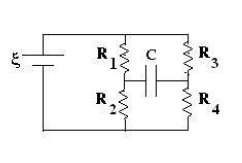
\includegraphics[width=\linewidth]{Problem_07_Figure.png}
\end{minipage}

\category{DC Circuits}
\StudyGuideLinks{7}
\ProblemSource{7}
\begin{answerbox}
\finalanswer{(D) 2.2 V}
\end{answerbox}
\begin{insightbox}
At steady state the capacitor branch is open; find node voltages by dividers and subtract them.
\end{insightbox}
\begin{solutionbox}

After a long time, the capacitor branch is open. Two independent dividers yield $V_A = 6\,\text{V}\cdot\tfrac{3}{7+3} = 1.8\,\text{V}$ and $V_B = 6\,\text{V}\cdot\tfrac{12}{6+12} = 4.0\,\text{V}$. Thus $V_C = |V_B-V_A| = 2.2\,\text{V}$.
\par\smallskip Equivalent node-voltage viewpoint: with the capacitor open, KCL at the top nodes gives the same divider values; the capacitor voltage is the node difference $|V_B-V_A|$.
\end{solutionbox}

% Problem 8
\Needspace{18\baselineskip}
\item \label{prob:8}
\noindent\begin{minipage}[t]{0.55\linewidth}
\vspace{0pt}
An electron moves in the plane of the page through two regions of space along the dotted-line trajectory shown in the figure. There is a uniform electric field in Region I directed into the plane of the page. There is no electric field in Region II. What is a necessary direction of the magnetic field in regions I and II? Ignore gravitational forces.
\begin{enumerate}[label=(\Alph*)]
    \item Region I: Downward along the page, Region II: Upward along the page
    \item Region I: Upward along the page, Region II: Into the page
    \item Region I: Upward along the page, Region II: Out of the page
    \item Region I: Downward along the page, Region II: Out of the page
    \item Region I: Into the page, Region II: Upward along the page
\end{enumerate}
\end{minipage}%
\hfill
\begin{minipage}[t]{0.4\linewidth}
\vspace{0pt}
\centering
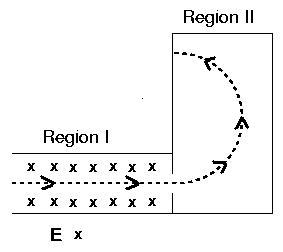
\includegraphics[width=\linewidth]{Problem_08_Figure.png}
\end{minipage}

\category{Electricity \& Magnetism}
\StudyGuideLinks{8}
\ProblemSource{8}
\begin{answerbox}
\finalanswer{(C) Region I: Upward along the page, Region II: Out of the page}
\end{answerbox}
\begin{insightbox}
Use $\vec F_B=q\,\vec v\times\vec B$ and the negative charge of an electron to choose the $\vec B$ directions that curve the trajectory as shown.
\end{insightbox}
\begin{solutionbox}

In Region I, $\vec F_E$ on the electron is out of the page, so $\vec F_B$ must be into the page; with $q<0$, this requires $\vec v\times\vec B$ out of the page, hence $\vec B$ upward along the page. In Region II, curvature upward along the page implies $\vec F_B$ upward along the page. With $q<0$ and $\vec v$ rightward, $\vec B$ is out of the page.
\end{solutionbox}

% Problem 9
\Needspace{18\baselineskip}
\item \label{prob:9}
\noindent\begin{minipage}[t]{0.6\linewidth}
\vspace{0pt}
For the circuit shown, when a shorting wire (no resistance) connects the points labeled A and B, which of the numbered light bulbs become brighter? Assume that all four bulbs are identical and have resistance R.
\begin{enumerate}[label=(\Alph*)]
    \item Bulb 1 only
    \item Bulb 2 only
    \item Bulb 3 only
    \item Bulbs 1 and 3 only
    \item Bulbs 1, 2, and 3
\end{enumerate}
\end{minipage}%
\hfill
\begin{minipage}[t]{0.33\linewidth}
\vspace{0pt}
\centering
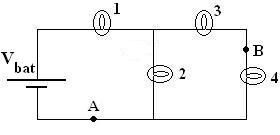
\includegraphics[width=\linewidth]{Problem_09_Figure.png}
\end{minipage}

\category{DC Circuits}
\StudyGuideLinks{9}
\ProblemSource{9} 
\begin{answerbox}
\finalanswer{(D) Bulbs 1 and 3 only}
\end{answerbox}
\begin{insightbox}
Shorting A to B bypasses bulb 4 and changes the currents in the remaining branches.
\end{insightbox}
\begin{solutionbox}

Label the left node at the bottom of the source A and the right mid node B (see figure). Bulbs 1 and 3 are on the top branches left and right of the central vertical branch containing bulb 2; bulb 4 is on the right outer branch.

Let the battery voltage be $V$. Initially bulb 1 is in series with bulb 2 in parallel with bulbs 3 and 4 in series. The equivalent resistance is $R+(R\parallel2R)=5R/3$. Thus $I_1=3V/(5R)$, $I_2=2V/(5R)$, and $I_3=I_4=V/(5R)$.

After A and B are connected, bulb 4 is shorted. Bulb 1 is in series with bulbs 2 and 3 in parallel, giving $R_{\rm eq}=3R/2$. The new currents are $I_1=2V/(3R)$, $I_2=I_3=V/(3R)$, and $I_4=0$. Because $P=I^2R$ for identical bulbs, bulbs 1 and 3 brighten; bulb 2 dims and bulb 4 goes out.
\end{solutionbox}

% Problem 10
\Needspace{18\baselineskip}
\item \label{prob:10}
A car moves to the right along a one-dimensional track for total time $T$ in two parts. Part One: The car maintains constant non-zero speed $V$ for the first $\tfrac{3}{4}$ of the total time. Part Two: The car accelerates uniformly to rest during the last $\tfrac{1}{4}$ of the total time. What is the ratio of the distance traveled during Part One of the trip to the distance traveled during Part Two of the trip?
\begin{enumerate}[label=(\Alph*)]
    \item 6:1
    \item 3:2
    \item The values of V and T are required to answer the question.
    \item 4:3
    \item 8:3
\end{enumerate}

\category{Kinematics}
\StudyGuideLinks{10}
\ProblemSource{10} 
\begin{answerbox}
\finalanswer{(A) 6:1}
\end{answerbox}
\begin{insightbox}
Distance 1: $V\cdot 3T/4$; distance 2: $(V/2)\cdot T/4$. Ratio is 6:1.
\end{insightbox}
\begin{solutionbox}

Part one: $d_1=V\cdot (3T/4)=\tfrac{3}{4}VT$. Part two (uniform decel from $V$ to 0 over $T/4$): $\bar v = V/2$, so $d_2=\bar v\cdot (T/4)=\tfrac{1}{8}VT$. So $d_1:d_2=6:1$.
\end{solutionbox}

% Problem 11
\Needspace{18\baselineskip}
\item \label{prob:11}
\noindent\begin{minipage}[t]{0.6\linewidth}
\vspace{0pt}
A piece of an ideal fluid is marked as it moves along a horizontal streamline through a pipe, as shown in the figure. In Region I, the speed of the fluid on the streamline is $V$. The cylindrical, horizontal pipe narrows so that the radius of the pipe in Region II is half of what it was in Region I. What is the speed of the marked fluid when it is in Region II?
\begin{enumerate}[label=(\Alph*)]
    \item 4$V$
    \item 2$V$
    \item $V$
    \item $V/2$
    \item $V/4$
\end{enumerate}
\end{minipage}%
\hfill
\begin{minipage}[t]{0.35\linewidth}
\vspace{0pt}
\centering
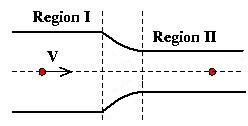
\includegraphics[width=\linewidth]{Problem_11_Figure.png}
\end{minipage}

\category{Fluid Mechanics}
\StudyGuideLinks{11}
\ProblemSource{11} 
\begin{answerbox}
\finalanswer{(A) 4V}
\end{answerbox}
\begin{insightbox}
Continuity $A_1v_1=A_2v_2$: halving the radius quarters the area, so the speed quadruples.
\end{insightbox}
\begin{solutionbox}

Continuity: $A_1 v_1 = A_2 v_2$ with $A\propto r^2$. If $r_2=\tfrac{1}{2}r_1$, then $A_2=\tfrac{1}{4}A_1$, so $v_2 = (A_1/A_2) v_1 = 4V$.
\end{solutionbox}

% Problem 12
\Needspace{18\baselineskip}
\item \label{prob:12}
\noindent\begin{minipage}[t]{0.6\linewidth}
\vspace{0pt}
For the RC circuit shown, the resistance is $R = 10.0 \Omega$, the capacitance is $C = 5.0\,\mathrm{F}$ and the battery has voltage $\mathcal E = 12$ volts. The capacitor is initially uncharged when the switch S is closed at time $t = 0$. At some time later, the current in the circuit is $0.50$ A. What is the magnitude of the voltage across the capacitor at that moment?
\begin{enumerate}[label=(\Alph*)]
    \item 0 volts
    \item 5 volts
    \item 6 volts
    \item 7 volts
    \item 12 volts
\end{enumerate}
\end{minipage}%
\hfill
\begin{minipage}[t]{0.35\linewidth}
\vspace{0pt}
\centering
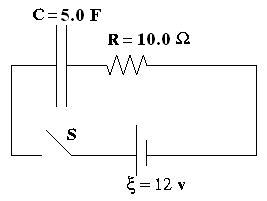
\includegraphics[width=\linewidth]{Problem_12_Figure.png}
\end{minipage}

\category{RC Circuits}
\StudyGuideLinks{12}
\ProblemSource{12}
\begin{answerbox}
\finalanswer{(D) 7 volts}
\end{answerbox}
\begin{insightbox}
KVL: $\mathcal E=V_R+V_C$. With $I$ known, find $V_R=IR$ then $V_C$.
\end{insightbox}
\begin{solutionbox}

KVL: $\mathcal E - V_R - V_C = 0$. With $I=0.50\,\text{A}$ and $R=10.0\,\Omega$, $V_R=IR=5.0\,\text{V}$. Hence $V_C=\mathcal E - V_R = 12-5=7\,\text{V}$.
\end{solutionbox}

% Problem 13
\Needspace{18\baselineskip}
\item \label{prob:13}
A ball initially at rest falls without air resistance from a height $h$ above the ground. If the ball falls the first distance $h/2$ in a time $t$, how much time is required to fall the remaining distance of $h/2$?
\begin{enumerate}[label=(\Alph*)]
    \item 0.25$t$
    \item 0.41$t$
    \item 0.50$t$
    \item 0.71$t$
    \item 1.00$t$
\end{enumerate}

\category{Kinematics}
\StudyGuideLinks{13}
\ProblemSource{13}
\begin{answerbox}
\finalanswer{(B) 0.41t}
\end{answerbox}
\begin{insightbox}
First half gives $h=gt^2$; total time is $\sqrt2 t$, so the remainder is $(\sqrt2-1)t\approx0.414t$.
\end{insightbox}
\begin{solutionbox}

With $d=\tfrac{1}{2}gt^2$, first half: $h/2=\tfrac{1}{2}gt^2\Rightarrow h=gt^2$. Total time $t_{\text{tot}}$ satisfies $h=\tfrac{1}{2}g t_{\text{tot}}^2\Rightarrow t_{\text{tot}}=\sqrt{2}t$. Remaining time $t_{\text{rem}}=t_{\text{tot}}-t=(\sqrt{2}-1)t\approx 0.414t$.
\end{solutionbox}

% Problem 14
\Needspace{18\baselineskip}
\item \label{prob:14}
\noindent\begin{minipage}[t]{0.6\linewidth}
\vspace{0pt}
An object of mass M starts from rest at the bottom of a fixed incline of height H. A person decides to push the object up the incline in one of two ways with an applied force shown in the diagram. In each of the trials, the object reaches the top of the incline with speed $V$. How would the work done by the person on the block compare for the two trials? Assume the same constant non-zero coefficient of kinetic friction.
\begin{enumerate}[label=(\Alph*)]
    \item More work would be done in Trial 1
    \item More work would be done in Trial 2
    \item The work would be equal for both trials
    \item Impossible to determine without knowing $V$.
    \item Impossible to determine without knowing $\mu_k$.
\end{enumerate}
\end{minipage}%
\hfill
\begin{minipage}[t]{0.35\linewidth}
\vspace{0pt}
\centering
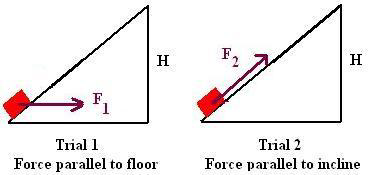
\includegraphics[width=\linewidth]{Problem_14_Figure.png}
\end{minipage}

\category{Work \& Energy with Friction}
\StudyGuideLinks{14}
\ProblemSource{14} 
\begin{answerbox}
\finalanswer{(A) More work would be done in Trial 1}
\end{answerbox}
\begin{insightbox}
A horizontal push raises the normal force and friction loss; since $\Delta K$ and $W_g$ match, external work must be larger.
\end{insightbox}
\begin{solutionbox}

Horizontal push increases the normal force: $N_1=Mg\cos\theta+F_1\sin\theta>Mg\cos\theta=N_2$, so friction is larger in Trial 1. Since $\Delta K$ and $W_g$ are the same, the greater friction loss requires more input work in Trial 1.
\end{solutionbox}

% Problem 15
\Needspace{18\baselineskip}
\item \label{prob:15}
\noindent\begin{minipage}[t]{0.6\linewidth}
\vspace{0pt}
A point object with mass $M=2.0$kg is attached a distance $R=1.75$m from the fixed center of a disk. The disk starts rotating from rest with constant angular acceleration $\alpha = 5.00$ rad/s$^2$. After how much time $T$ (in seconds) is the tangential acceleration equal in magnitude to the centripetal acceleration?
\begin{enumerate}[label=(\Alph*)]
    \item 0.769
    \item 0.592
    \item 0.500
    \item 0.447
    \item 0.350
\end{enumerate}
\end{minipage}%
\hfill
\begin{minipage}[t]{0.35\linewidth}
\vspace{0pt}
\centering
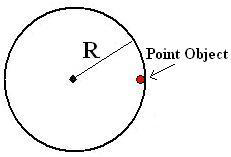
\includegraphics[width=\linewidth]{Problem_15_Figure.png}
\end{minipage}

\category{Rotational Kinematics}
\StudyGuideLinks{15}
\ProblemSource{15} 
\begin{answerbox}
\finalanswer{(D) 0.447}
\end{answerbox}
\begin{insightbox}
Set $a_t=R\alpha$ equal to $a_c=R(\alpha T)^2$ to get $T=1/\sqrt{\alpha}$.
\end{insightbox}
\begin{solutionbox}

Set $a_t=R\alpha$ equal to $a_c=R\omega^2=R(\alpha T)^2$. Then $R\alpha=R\alpha^2 T^2\Rightarrow T=1/\sqrt{\alpha}=1/\sqrt{5}\approx0.447\,\text{s}$.
\end{solutionbox}

% Problem 16
\Needspace{18\baselineskip}
\item \label{prob:16}
\noindent\begin{minipage}[t]{0.6\linewidth}
\vspace{0pt}
A uniform, solid cylinder with a mass M and radius R is pulled by a horizontal force F acting through the center as shown. The cylinder rolls to the right without slipping. What is the magnitude of the force of friction between the cylinder and the ground?
\begin{enumerate}[label=(\Alph*)]
    \item $\frac{1}{4}F$
    \item $\frac{1}{3}F$
    \item $\frac{1}{2}F$
    \item $\frac{2}{3}F$
    \item $\frac{3}{4}F$
\end{enumerate}
\end{minipage}%
\hfill
\begin{minipage}[t]{0.35\linewidth}
\vspace{0pt}
\centering
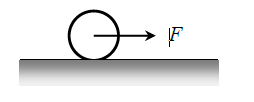
\includegraphics[width=\linewidth]{Problem_16_Figure.png}
\end{minipage}

\category{Rolling Dynamics}
\StudyGuideLinks{16}
\ProblemSource{16} 
\begin{answerbox}
\finalanswer{(B) $\tfrac{1}{3}F$}
\end{answerbox}
\begin{insightbox}
Combine translation $F-f=Ma$ with rotation $fR=I\alpha$ and $a=R\alpha$ to obtain $f=F/3$.
\end{insightbox}
\begin{solutionbox}

Translational: $F-f=Ma$. Rotational: $fR=I\alpha$ with $I=\tfrac{1}{2}MR^2$ and $a=R\alpha$. Then $f=\tfrac{1}{2}Ma$. Sub into translation: $F-f=2f\Rightarrow F=3f\Rightarrow f=F/3$.
\end{solutionbox}

% Problem 17
\Needspace{18\baselineskip}
\item \label{prob:17}
A comet moves in an elliptical orbit around the sun. As the comet moves from aphelion (farthest point) to perihelion (closest point), which of the following results is true?
\begin{enumerate}[label=(\Alph*)]
    \item Speed of the comet: Increases, Angular momentum of the comet/sun system: Increases, Gravitational potential energy of the comet/sun system: Decreases
    \item Speed of the comet: Increases, Angular momentum of the comet/sun system: Constant, Gravitational potential energy of the comet/sun system: Decreases
    \item Speed of the comet: Decreases, Angular momentum of the comet/sun system: Decreases, Gravitational potential energy of the comet/sun system: Increases
    \item Speed of the comet: Increases, Angular momentum of the comet/sun system: Increases, Gravitational potential energy of the comet/sun system: Constant
    \item Speed of the comet: Constant, Angular momentum of the comet/sun system: Constant, Gravitational potential energy of the comet/sun system: Constant
\end{enumerate}

\category{Gravitation}
\StudyGuideLinks{17}
\ProblemSource{17} 
\begin{answerbox}
\finalanswer{(B) Increases, Constant, Decreases}
\end{answerbox}
\begin{insightbox}
Zero torque about the sun conserves angular momentum; as $r$ decreases, $U=-GMm/r$ drops and speed rises.
\end{insightbox}
\begin{solutionbox}

Central gravity gives zero torque, so angular momentum is conserved. As $r$ decreases, $U=-GMm/r$ decreases, hence kinetic energy and speed increase.
\end{solutionbox}

% Problem 18
\Needspace{18\baselineskip}
\item \label{prob:18}
\noindent\begin{minipage}[t]{0.6\linewidth}
\vspace{0pt}
An open cylindrical container with very large radius is at rest a distance $H$ above the ground at the edge of a platform. A tiny hole develops at the bottom of the container and water from the container squirts out horizontally landing a distance $H$ from the edge of the platform. For the water to land at this location, what is the depth of the water $L$ in the container? The figure is not drawn to scale and air resistance is ignored.
\begin{enumerate}[label=(\Alph*)]
    \item $H/4$
    \item $H/\sqrt{2}$
    \item $H$
    \item $H\sqrt{2}$
    \item $2H$
\end{enumerate}
\end{minipage}%
\hfill
\begin{minipage}[t]{0.32\linewidth}
\vspace{0pt}
\centering
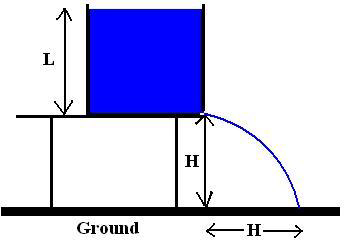
\includegraphics[width=\linewidth]{Problem_18_Figure.png}
\end{minipage}

\category{Fluid Mechanics \& Projectile Motion}
\StudyGuideLinks{18}
\ProblemSource{18} 
\begin{answerbox}
\finalanswer{(A) $H/4$}
\end{answerbox}
\begin{insightbox}
Torricelli gives $v=\sqrt{2gL}$; range $H$ equals $v$ times fall time $\sqrt{2H/g}$.
\end{insightbox}
\begin{solutionbox}

Torricelli: $v=\sqrt{2gL}$. Time of fall from height $H$ is $t=\sqrt{2H/g}$. Range $H=v t=\sqrt{2gL}\,\sqrt{2H/g}=\sqrt{4LH}$. Hence $H^2=4LH\Rightarrow L=H/4$.
\end{solutionbox}

% Problem 19
\Needspace{18\baselineskip}
\item \label{prob:19}
\noindent\begin{minipage}[t]{0.6\linewidth}
\vspace{0pt}
A monatomic ideal gas is the working substance for an engine that undergoes the cyclic process (ABCDA) shown in the PV diagram. The processes are all isochoric or isobaric with pressures between $P_0$ and $2P_0$ and volumes between $V_0$ and $\frac{3}{2}V_0$. What is the efficiency of this engine?
\begin{enumerate}[label=(\Alph*)]
    \item $1/8$
    \item $1/5$
    \item $1/3$
    \item $2/3$
    \item $5/7$
\end{enumerate}
\end{minipage}%
\hfill
\begin{minipage}[t]{0.32\linewidth}
\vspace{0pt}
\centering
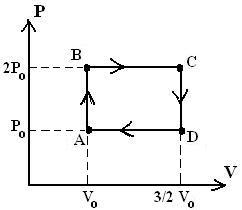
\includegraphics[width=\linewidth]{Problem_19_Figure.png}
\end{minipage}

\category{Thermodynamics \& Engines}
\StudyGuideLinks{19}
\ProblemSource{19} 
\begin{answerbox}
\finalanswer{(A) 1/8}
\end{answerbox}
\begin{insightbox}
Compute heat on isobaric/isochoric legs; net work is rectangle area $\Delta P\,\Delta V$; efficiency is $W/Q_{in}$. Sign guide: isobaric expansion (heat in, $W>0$), isochoric heating (heat in, $W=0$), isobaric compression (heat out, $W<0$), isochoric cooling (heat out, $W=0$).
\end{insightbox}
\begin{solutionbox}

Net work: $W=\Delta P\,\Delta V= (2P_0-P_0)\,(\tfrac{3}{2}V_0-V_0)=\tfrac{1}{2}P_0V_0$. Heat in during AB and BC: $Q_{in}=\tfrac{3}{2}P_0V_0+\tfrac{5}{2}P_0V_0=4P_0V_0$. Efficiency $\eta=W/Q_{in}=1/8$.
\end{solutionbox}

% Problem 20
\Needspace{18\baselineskip}
\item \label{prob:20}
\noindent\begin{minipage}[t]{0.6\linewidth}
\vspace{0pt}
A solid, uniform sphere rolls without slipping on a floor along the +x-axis. The rotational kinetic energy associated with the sphere about an axis through its center of mass along the +z-axis is 20 Joules. What is the translational kinetic energy associated with the sphere?
\begin{enumerate}[label=(\Alph*)]
    \item 8 J
    \item 10 J
    \item 20 J
    \item 40 J
    \item 50 J
\end{enumerate}
\end{minipage}%
\hfill
\begin{minipage}[t]{0.32\linewidth}
\vspace{0pt}
\centering
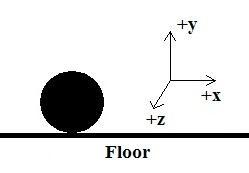
\includegraphics[width=\linewidth]{Problem_20_Figure.png}
\end{minipage}

\category{Rolling Energy}
\StudyGuideLinks{20}
\ProblemSource{20} 
\begin{answerbox}
\finalanswer{(E) 50 J}
\end{answerbox}
\begin{insightbox}
With pure rolling $v=R\omega$, a solid sphere has $K_{rot}=\tfrac{1}{5}mv^2$, so $K_{trans}=(5/2)K_{rot}$.
\end{insightbox}
\begin{solutionbox}

For a solid sphere, $I=\tfrac{2}{5}mR^2$ and $v=R\omega$. Then $K_{rot}=\tfrac{1}{2}I\omega^2=\tfrac{1}{5}mv^2$. Meanwhile $K_{trans}=\tfrac{1}{2}mv^2=\tfrac{5}{2}K_{rot}=50\,\text{J}$.
\end{solutionbox}

% Problem 21
\Needspace{18\baselineskip}
\item \label{prob:21}
A student wants to set up an experiment with a thin convex lens of focal length $f$ such that a thin real object produces a focused real image on a movable screen. At how many locations along the optical axis can the object be placed so that the distance between the object and the focused image on the screen is equal to $3f$?
\begin{enumerate}[label=(\Alph*)]
    \item There is no location.
    \item There is exactly one location.
    \item There are exactly two locations.
    \item There are exactly four locations.
    \item There are an infinite number of locations.
\end{enumerate}

\category{Geometric Optics}
\StudyGuideLinks{21}
\ProblemSource{21}
\begin{answerbox}
\finalanswer{(A) There is no location.}
\end{answerbox}
\begin{insightbox}
Solve $1/d_o+1/d_i=1/f$ with $d_o+d_i=3f$; the quadratic has negative discriminant, so no real location. Only when the object–image separation $D\ge 4f$ can a real solution exist.
\end{insightbox}
\begin{solutionbox}

With $\tfrac{1}{d_o}+\tfrac{1}{d_i}=\tfrac{1}{f}$ and $D=d_o+d_i=3f$, substitute $d_i=3f-d_o$:
\[
\frac{1}{d_o}+\frac{1}{3f-d_o}=\frac{1}{f} \Rightarrow d_o^2-3fd_o+3f^2=0.
\]
Discriminant $\Delta=9f^2-12f^2=-3f^2<0$, so no real $d_o$ exists.
\end{solutionbox}

% Problem 22
\Needspace{18\baselineskip}
\item \label{prob:22}
\noindent\begin{minipage}[t]{0.6\linewidth}
\vspace{0pt}
For the circuit shown, all wires have no resistance, the battery has a constant internal resistance of $r = 8.0\,\Omega$ and the two light bulbs are identical. The variable resistor is initially set to $R = 26.0\,\Omega$. The switch S is closed. To what resistance must the variable resistor be set if bulb \#1 is to have the same brightness after the switch is closed as it did with the switch open?
\begin{enumerate}[label=(\Alph*)]
    \item $9.0\,\Omega$
    \item $13.0\,\Omega$
    \item $18.0\,\Omega$
    \item $22.0\,\Omega$
    \item The answer can be computed only if the bulbs’ resistance is known.
\end{enumerate}
\end{minipage}%
\hfill
\begin{minipage}[t]{0.32\linewidth}
\vspace{0pt}
\centering
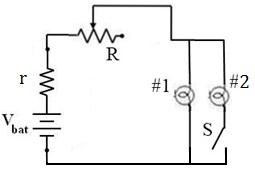
\includegraphics[width=\linewidth]{Problem_21_Figure.png}
\end{minipage}

\category{DC Circuits}
\StudyGuideLinks{22}
\ProblemSource{22}
\begin{answerbox}
\finalanswer{(A) $9.0\,\Omega$}
\end{answerbox}
\begin{insightbox}
Keep bulb 1 current unchanged; equate open/closed currents in the equivalent circuits to solve $R'$.
\end{insightbox}
\begin{solutionbox}

Open: $I_{1,\text{open}}=\tfrac{\mathcal E}{r+R_b+R}$. Closed: bulbs in parallel $R_p=R_b/2$, total $r+R_b/2+R'$, current splits equally so $I_{1,\text{closed}}=\tfrac{\mathcal E}{2r+R_b+2R'}$. Equate:
\[
r+R_b+R=2r+R_b+2R' \Rightarrow R' = \tfrac{R-r}{2} = \tfrac{26-8}{2}=9.0\,\Omega.
\]
\end{solutionbox}

% Problem 23
\Needspace{18\baselineskip}
\item \label{prob:23}
\noindent\begin{minipage}[t]{0.6\linewidth}
\vspace{0pt}
A mass on a frictionless incline has a gravitational force, a normal force, and an applied force that all are equal in magnitude. The mass remains at rest. The incline makes an angle $\theta$ with the horizontal. Which one of the following choices best describes the orientation of the applied force? The +x-axis is parallel to the incline’s surface.
\begin{enumerate}[label=(\Alph*)]
    \item Oriented directly along the +x axis.
    \item Oriented at an angle $\theta$ clockwise from the +x axis.
    \item Oriented at an angle $90^\circ - \theta$ clockwise from the +x axis.
    \item Oriented at an angle $90^\circ - \theta$ counterclockwise from the +x axis.
    \item This is a completely impossible situation.
\end{enumerate}
\end{minipage}%
\hfill
\begin{minipage}[t]{0.32\linewidth}
\vspace{0pt}
\centering
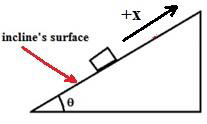
\includegraphics[width=\linewidth]{Problem_23_Figure.png}
\end{minipage}

\category{Statics}
\StudyGuideLinks{23}
\ProblemSource{23}
\begin{answerbox}
\finalanswer{(C) Oriented at $90^\circ-\theta$ clockwise from +x}
\end{answerbox}
\begin{insightbox}
Resolve the applied force along and perpendicular to the incline, then use its given magnitude.
\end{insightbox}
\begin{solutionbox}
The force components needed for equilibrium are $F_{a,x}=mg\sin\theta$ and $F_{a,y}=mg(\cos\theta-1)$. Since $F_a=mg$, their squared magnitudes give $2(1-\cos\theta)=1$, hence $\theta=60^\circ$ for an incline. The applied force is therefore $30^\circ=90^\circ-\theta$ clockwise from the $+x$ axis. The stated equal-force condition itself fixes the incline angle.
\end{solutionbox}

% Problem 24
\Needspace{18\baselineskip}
\item \label{prob:24}
The position of a mass connected to a spring obeys $x(t) = A \cos(\omega t)$. What is the average speed of the mass for one full oscillation in terms of the mass’s maximum speed during oscillation, $v_{max}$?
\begin{enumerate}[label=(\Alph*)]
    \item $\frac{2}{\pi} v_{max}$
    \item $\frac{1}{\sqrt{2}} v_{max}$
    \item $\frac{1}{2} v_{max}$
    \item $\frac{\sqrt{2}}{\pi} v_{max}$
    \item $\frac{1}{2\pi\sqrt{2}} v_{max}$
\end{enumerate}

\category{Oscillations}
\StudyGuideLinks{24}
\ProblemSource{24}
\begin{answerbox}
\finalanswer{(A) $\tfrac{2}{\pi}v_{max}$}
\end{answerbox}
\begin{insightbox}
In one period distance is $4A$, $T=2\pi/\omega$, and $v_{max}=A\omega$; substitute to get $\bar s=(2/\pi)v_{max}$.
\end{insightbox}
\begin{solutionbox}

During one period $T=2\pi/\omega$, distance covered is $4A$. With $v_{max}=A\omega$, the average speed is $\bar s=4A/T=2A\omega/\pi=\tfrac{2}{\pi}v_{max}$.
\end{solutionbox}

% Problem 25
\Needspace{18\baselineskip}
\item \label{prob:25}
\noindent\begin{minipage}[t]{0.6\linewidth}
\vspace{0pt}
An upward-pointing object is placed 15.0 cm to the left of a lens system. The first lens is convex with focal length 10.0 cm. The second lens is convex with focal length 10 cm and its location from the first lens is varied from $x=10$ cm away to $x=110$ cm away. Which one of the following choices best represents the description of the final image formed as the second lens is moved from $x=10$ cm to $x=110$ cm from the first lens?
\end{minipage}%
\hfill
\begin{minipage}[t]{0.32\linewidth}
\vspace{0pt}
\centering
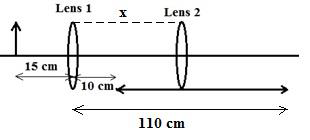
\includegraphics[width=\linewidth]{Problem_26_Figure.png}
\end{minipage}

\begin{enumerate}[label=(\Alph*)]
    \item $x=10$ cm away: Real \& pointing downward; $\quad x=110$ cm away: Real \& pointing upward
    \item $x=10$ cm away: Virtual \& pointing downward; $\quad x=110$ cm away: Real \& pointing upward
    \item $x=10$ cm away: Virtual \& pointing upward; $\quad x=110$ cm away: Real \& pointing downward
    \item $x=10$ cm away: Real \& pointing upward; $\quad x=110$ cm away: Real \& pointing upward
    \item $x=10$ cm away: Virtual \& pointing downward; $\quad x=110$ cm away: Virtual \& pointing downward
\end{enumerate}

\category{Geometric Optics}
\StudyGuideLinks{25}
\ProblemSource{25}
\begin{answerbox}
\finalanswer{(A) Real \& pointing downward at $x=10$ cm; Real \& pointing upward at $x=110$ cm.}
\end{answerbox}
\begin{insightbox}
The image of the first lens is the object for the second; its signed distance changes as the second lens moves.
\end{insightbox}
\begin{solutionbox}
\textbf{Behavior vs. $x$:} The final image is real and inverted for $10\le x<30$, becomes virtual and inverted for $30<x<40$, and is real and upright for $x>40$. At $x=30$ the intermediate image lies in the second lens plane, so the usual object-distance formula is singular; at $x=40$ the image lies at infinity.

Using $d_{i1}=30\,\text{cm}$ from lens 1, the second lens has $d_{o2}=x-30$. With $f_2=10$ cm,
\[ d_{i2}=\frac{10(x-30)}{x-40}, \quad m_{\text{total}}=\frac{20}{x-40}. \]
Signs of $d_{i2}$ and $m_{\text{total}}$ across intervals give the stated behavior.
\end{solutionbox}

% Problem 26
\Needspace{18\baselineskip}
\item \label{prob:26}
Rain falls vertically at 12.0 m/s in the ground frame. A car travels down a slope at $40^\circ$ below the horizontal. A passenger sees the rain moving at $29.0^\circ$ from vertical. What is the car's speed relative to the ground?
\begin{enumerate}[label=(\Alph*)]
    \item 2.29 m/s
    \item 5.93 m/s
    \item 9.03 m/s
    \item 11.8 m/s
    \item 16.2 m/s
\end{enumerate}

\category{Relative Motion}
\StudyGuideLinks{26}
\ProblemSource{26}
\begin{answerbox}
\finalanswer{(B) $5.93\,\text{m/s}$}
\end{answerbox}
\begin{insightbox}
Subtract the car's velocity from the rain's velocity in both horizontal and vertical components.
\end{insightbox}
\begin{solutionbox}

Take right and up as positive. The rain has $\vec v_{r/g}=(0,-12)$ and the car has $\vec v_{c/g}=(v_c\cos40^\circ,-v_c\sin40^\circ)$. Thus $\vec v_{r/c}=(-v_c\cos40^\circ,-12+v_c\sin40^\circ)$. The passenger's observation gives
\[
\tan29^\circ=\frac{v_c\cos40^\circ}{12-v_c\sin40^\circ}
\quad\Rightarrow\quad
v_c=\frac{12\tan29^\circ}{\cos40^\circ+\sin40^\circ\tan29^\circ}
\approx5.93\,\mathrm{m/s}.
\]
\emph{Editorial note:} The earlier repository transcription contained conflicting directions. The slope and $29^\circ$ observation above follow the original 2015 problem.
\end{solutionbox}

% Problem 27
\Needspace{18\baselineskip}
\item \label{prob:27}
\noindent\begin{minipage}[t]{0.6\linewidth}
\vspace{0pt}
A 2.0 kg mass is connected to the end of string and moves about the string’s fixed end in a conical motion with a constant speed of 4.0 m/s. The string has a length of 2.50 m and forms an angle of $\theta$ with the vertical. Use $g=10\,\mathrm{m/s^2}$. What is the tension in the string?
\begin{enumerate}[label=(\Alph*)]
    \item 20.0 N
    \item 23.7 N
    \item 27.4 N
    \item 29.8 N
    \item 32.5 N
\end{enumerate}
\end{minipage}%
\hfill
\begin{minipage}[t]{0.35\linewidth}
\vspace{0pt}
\centering
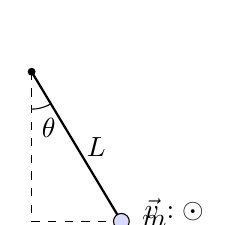
\begin{tikzpicture}[scale=0.95,>=Stealth]
  \coordinate (pivot) at (0,2);
  \coordinate (mass) at (1.2,0);
  \draw[dashed] (pivot) -- (0,0) -- (mass);
  \draw[thick] (pivot) -- (mass) node[midway,right] {$L$};
  \fill (pivot) circle (1.5pt);
  \filldraw[fill=blue!15] (mass) circle (3pt) node[right=4pt] {$m$};
  \draw (0,1.5) arc[start angle=-90,end angle=-59,radius=.5];
  \node at (.23,1.25) {$\theta$};
  \node[right] at (1.38,.16) {$\vec v:\odot$};
\end{tikzpicture}
\end{minipage}

\category{Circular Motion}
\StudyGuideLinks{27}
\ProblemSource{27}
\begin{answerbox}
\finalanswer{(C) 27.4 N}
\end{answerbox}
\begin{insightbox}
Use vertical equilibrium and horizontal centripetal acceleration, with the circular radius $r=L\sin\theta$.
\end{insightbox}
\begin{solutionbox}

From $T\cos\theta=mg$ and $T\sin\theta=mv^2/(L\sin\theta)$, eliminate $\theta$:
\[
 T-\frac{(mg)^2}{T}=\frac{mv^2}{L}=12.8\,\mathrm N.
\]
The positive root of $T^2-12.8T-400=0$ is $T\approx27.4\,\mathrm N$.
\end{solutionbox}

% Problem 28
\Needspace{18\baselineskip}
\item \label{prob:28}
\noindent\begin{minipage}[t]{0.6\linewidth}
\vspace{0pt}
A box slides with uniform acceleration up an incline. The box has an initial speed of 9.0 m/s and rises vertically 2.60 m before coming to rest. Use $g=10\,\mathrm{m/s^2}$. If the angle of the incline is $30^\circ$, what is the coefficient of kinetic friction between the box and the incline?
\begin{enumerate}[label=(\Alph*)]
    \item 0.298
    \item 0.322
    \item 0.372
    \item 0.483
    \item 0.557
\end{enumerate}
\end{minipage}%
\hfill
\begin{minipage}[t]{0.35\linewidth}
\vspace{0pt}
\centering
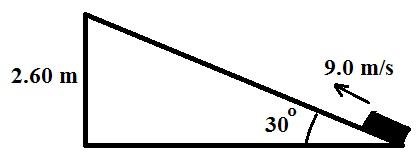
\includegraphics[width=\linewidth]{Problem_28_Figure.png}
\end{minipage}

\category{Work \& Energy with Friction}
\StudyGuideLinks{28}
\ProblemSource{28}
\begin{answerbox}
\finalanswer{(B) 0.322}
\end{answerbox}
\begin{insightbox}
The initial kinetic energy becomes gravitational potential energy and thermal energy from friction.
\end{insightbox}
\begin{solutionbox}

Energy lost to friction is positive on the right-hand side:
\[
\tfrac12 mv^2=mgh+\mu_k mg\cos30^\circ\,d,
\qquad d=\frac{2.60}{\sin30^\circ}=5.20\,\mathrm m.
\]
Therefore $\mu_k=(40.5-26.0)/(10\cos30^\circ\cdot5.20)\approx0.322$.
\end{solutionbox}

% Problem 29
\Needspace{18\baselineskip}
\item \label{prob:29}
\noindent\begin{minipage}[t]{0.6\linewidth}
\vspace{0pt}
A 9.20 m long uniform plank rests on a frictionless ice pond. A 52 kg box rests on the plank’s left end while a 71 kg person stands at the plank’s right end. After the person walks to the left on the plank and stands at the same location as the box, the plank has slid 3.84 m to the right relative to the pond’s shore. Which one of the following choices best represents the mass of the plank?
\begin{enumerate}[label=(\Alph*)]
    \item 123 kg
    \item 61.5 kg
    \item 47.1 kg
    \item 36.5 kg
    \item 31.2 kg
\end{enumerate}
\end{minipage}%
\hfill
\begin{minipage}[t]{0.35\linewidth}
\vspace{0pt}
\centering
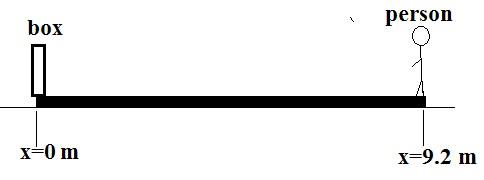
\includegraphics[width=\linewidth]{Problem_29_Figure.png}
\end{minipage}

\category{Center of Mass}
\StudyGuideLinks{29}
\ProblemSource{29}
\begin{answerbox}
\finalanswer{(C) 47.1 kg}
\end{answerbox}
\begin{insightbox}
No external horizontal force acts, so the horizontal center of mass remains fixed.
\end{insightbox}
\begin{solutionbox}

Stationary center of mass: $M_p\Delta x_p+M_b\Delta x_b+M_{pers}\Delta x_{pers}=0$. With given displacements, $3.84M_p+199.68-380.56=0 \Rightarrow M_p\approx47.1\,\text{kg}$.
\end{solutionbox}

% Problem 30
\Needspace{18\baselineskip}
\item \label{prob:30}
At the top of a high cliff, a small rock is dropped from rest. A ball is launched straight downward with an initial speed of 36.0 m/s at a time of 2.10 s after the rock was dropped. Use $g=10\,\mathrm{m/s^2}$. When the ball has fallen 28.0 m further than the initially dropped rock, what is the speed of the ball relative to the rock?
\begin{enumerate}[label=(\Alph*)]
    \item 15.0 m/s
    \item 16.0 m/s
    \item 20.0 m/s
    \item 21.0 m/s
    \item 36.0 m/s
\end{enumerate}

\category{Kinematics}
\StudyGuideLinks{30}
\ProblemSource{30}
\begin{answerbox}
\finalanswer{(A) 15.0 m/s}
\end{answerbox}
\begin{insightbox}
Once both objects are in flight their accelerations match, so their relative velocity is constant.
\end{insightbox}
\begin{solutionbox}

Downward speeds: $v_r=gt$, $v_b=36+g(t-2.10)$ for $t\ge2.10$. Relative speed $v_{rel}=v_b-v_r=36-g\cdot2.10\approx15.0\,\text{m/s}$ (using $g\approx10\,\text{m/s}^2$).
\end{solutionbox}

% Problem 31
\Needspace{18\baselineskip}
\item \label{prob:31}
A mass that is in simple harmonic motion obeys the following position versus time equation: $y(t)=0.50\,\mathrm{m}\,\sin\big[(\pi/2)\,t\big]$ where $t$ is in seconds. What is the period of vibration of this mass?
\begin{enumerate}[label=(\Alph*)]
    \item 1.0 s
    \item 2.0 s
    \item 3.0 s
    \item 4.0 s
    \item 5.0 s
\end{enumerate}

\category{Oscillations}
\StudyGuideLinks{31}
\ProblemSource{31} 
\begin{answerbox}
\finalanswer{(D) 4.0 s}
\end{answerbox}
\begin{insightbox}
With $\omega=\pi/2$, $T=2\pi/\omega=4$ s.
\end{insightbox}
\begin{solutionbox}

Identify $\omega=\pi/2$. Then $T=2\pi/\omega=4.0\,\text{s}$.
\end{solutionbox}

% Problem 32
\Needspace{18\baselineskip}
\item \label{prob:32}
A particle has a total energy of 500 MeV and a linear momentum of 300 MeV/c. What is the mass of the particle?
\begin{enumerate}[label=(\Alph*)]
    \item 800 MeV/c$^2$
    \item 583 MeV/c$^2$
    \item 400 MeV/c$^2$
    \item 267 MeV/c$^2$
    \item 200 MeV/c$^2$
\end{enumerate}

\category{Modern Physics}
\StudyGuideLinks{32}
\ProblemSource{32}
\begin{answerbox}
\finalanswer{(C) 400 MeV/c$^2$}
\end{answerbox}
\begin{insightbox}
Relate total energy, momentum and rest energy using $E^2=(pc)^2+(mc^2)^2$.
\end{insightbox}
\begin{solutionbox}

$E^2=(pc)^2+(m_0c^2)^2$: $(500)^2=(300)^2+(m_0c^2)^2 \Rightarrow m_0c^2=\sqrt{160000}=400\,\text{MeV}$.
\end{solutionbox}

% Problem 33
\Needspace{18\baselineskip}
\item \label{prob:33}
Water flows out of a horizontal drainpipe at the rate of 120 kg per minute. Its initial vertical velocity is zero and it falls 3.20 m to the ground. Use $g=10\,\mathrm{m/s^2}$. What is the average force it exerts when it hits the ground?
\begin{enumerate}[label=(\Alph*)]
    \item 6.0 N
    \item 10.0 N
    \item 12.0 N
    \item 16.0 N
    \item 20.0 N
\end{enumerate}

\category{Momentum \& Impulse}
\StudyGuideLinks{33}
\ProblemSource{33}
\begin{answerbox}
\finalanswer{(D) 16.0 N}
\end{answerbox}
\begin{insightbox}
Find the water's downward speed immediately before impact, then use its vertical momentum flux.
\end{insightbox}
\begin{solutionbox}

Assume the water has negligible vertical velocity after striking the ground. The mass flow rate is $\dot m=120/60=2.0\,\text{kg/s}$ and the impact speed is $v=\sqrt{2gh}=8.0\,\text{m/s}$. The downward momentum flux gives an average force $F=\dot m\,v=16.0\,\text{N}$.
\end{solutionbox}

% Problem 34
\Needspace{18\baselineskip}
\item \label{prob:34}
Let M represent the magnification of an image. For which of the following arrangements of an object and an optical device would $-1 < M < 0$? 
\begin{enumerate}[label=(\Alph*)]
    \item The object is placed less than one focal length in front of a converging mirror.
    \item The object is placed between one focal length and two focal lengths in front of a diverging mirror.
    \item The object is placed less than one focal length in front of a diverging lens.
    \item The object is placed more than two focal lengths in front of a converging lens.
    \item The object is placed between one focal length and two focal lengths in front of a plane mirror.
\end{enumerate}

\category{Geometric Optics}
\StudyGuideLinks{34}
\ProblemSource{34} 
\begin{answerbox}
\finalanswer{(D) Converging lens with $d_o>2f$}
\end{answerbox}
\begin{insightbox}
A negative magnification means an inverted image; magnitude below one means a reduced image.
\end{insightbox}
\begin{solutionbox}

This produces a real, inverted, reduced image: $M=-d_i/d_o$ with $f<d_i<2f<d_o$, so $-1<M<0$.
\end{solutionbox}

% Problem 35
\Needspace{18\baselineskip}
\item \label{prob:35}
Two cars start from rest at the same position and move in the same direction. Car 1 accelerates at $a_1=3.0$ m/s$^2$. Two seconds later, Car 2 accelerates at $a_2=12.0$ m/s$^2$. How much time after Car 1 starts will Car 2 pass Car 1?
\begin{enumerate}[label=(\Alph*)]
    \item 3.0 s
    \item 4.0 s
    \item 5.0 s
    \item 6.0 s
    \item 7.0 s
\end{enumerate}

\category{Kinematics}
\StudyGuideLinks{35}
\ProblemSource{35} 
\begin{answerbox}
\finalanswer{(B) 4.0 s}
\end{answerbox}
\begin{insightbox}
Set $x_1=x_2$: $1.5t^2=6(t-2)^2$ and take the smallest $t\ge2$.
\end{insightbox}
\begin{solutionbox}

Positions: $x_1=1.5t^2$, $x_2=6(t-2)^2$ for $t\ge2$. Solve $1.5t^2=6(t-2)^2 \Rightarrow t=4.0$ s.
\end{solutionbox}

% Problem 36
\Needspace{18\baselineskip}
\item \label{prob:36}
\noindent\begin{minipage}[t]{0.6\linewidth}
\vspace{0pt}
Two boxes are stacked on a table as shown at right. The mass of box 1 is $m$ and the mass of box 2 is $3m$. The surface between box 2 and the table is smooth and the surface between the two boxes is rough. When a force, F, is applied, box 1 does not slide on box 2. What is the minimum coefficient of static friction between the boxes?
\begin{enumerate}[label=(\Alph*)]
    \item $F/(4mg)$
    \item $F/(3mg)$
    \item $F/(2mg)$
    \item $F/(mg)$
    \item $2mg/F$
\end{enumerate}
\end{minipage}%
\hfill
\begin{minipage}[t]{0.35\linewidth}
\vspace{0pt}
\centering
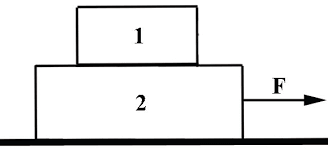
\includegraphics[width=\linewidth]{Problem_31_Figure.png}
\end{minipage}

\category{Dynamics \& Friction}
\StudyGuideLinks{36}
\ProblemSource{36} 
\begin{answerbox}
\finalanswer{(A) $F/(4mg)$}
\end{answerbox}
\begin{insightbox}
Overall acceleration $a=F/(4m)$; the top box requires static friction $F/4$. Compare with $\mu_s mg$ to get the minimum $\mu_s$.
\end{insightbox}
\begin{solutionbox}

Treating both boxes as one: $a=F/(4m)$. For the top box, required static friction $f_s=m a=F/4$. The maximum static friction is $\mu_s mg$, so $F/4\le \mu_s mg \Rightarrow \mu_s=F/(4mg)$.
\end{solutionbox}

% Problem 37
\Needspace{18\baselineskip}
\item \label{prob:37}
A uniform wooden block is a rectangular prism with dimensions of 10 cm x 6 cm x 2 cm. The block will be placed on a level table in one of three possible orientations with a side parallel to the tabletop. Let $P_L$ equal the largest possible pressure the block can exert on the table and $P_S$ equal the smallest possible pressure the block can exert on the table. What is the ratio $P_L/P_S$? 
\begin{enumerate}[label=(\Alph*)]
    \item 5/3
    \item 3
    \item 5
    \item 9
    \item 25
\end{enumerate}

\category{Statics}
\StudyGuideLinks{37}
\ProblemSource{37} 
\begin{answerbox}
\finalanswer{(C) 5}
\end{answerbox}
\begin{insightbox}
Pressure is inversely proportional to contact area; among the three faces the area ratio max/min is $60/12$.
\end{insightbox}
\begin{solutionbox}

Pressure $P=F/A$ with constant weight. Areas: 60, 20, 12 cm$^2$. Ratio $P_L/P_S=A_{max}/A_{min}=60/12=5$.
\end{solutionbox}

% Problem 38
\Needspace{18\baselineskip}
\item \label{prob:38}
A motorcycle has a total mass of 150 kg. Each wheel has a mass of 10 kg and a radius of 30 cm. As the motorcycle is moving, what is the ratio of the rotational kinetic energy of the wheels to the total translational kinetic energy of the motorcycle? Assume the wheels are uniform disks and roll without slipping.
\begin{enumerate}[label=(\Alph*)]
    \item 0.033:1
    \item 0.067:1
    \item 0.33:1
    \item 0.67:1
    \item 3.3:1
\end{enumerate}

\category{Rotational Energy}
\StudyGuideLinks{38}
\ProblemSource{38}
\begin{answerbox}
\finalanswer{(B) $0.067:1$}
\end{answerbox}
\begin{insightbox}
Compare the two wheels' combined rotational energy with the translation of the entire motorcycle.
\end{insightbox}
\begin{solutionbox}
Each wheel (uniform disk) has $I=\tfrac{1}{2}m_w R^2$ and rolls without slipping, so $\omega=v/R$. Thus one wheel's rotational energy is
\[
K_{\text{rot, one}}=\tfrac{1}{2}I\omega^2=\tfrac{1}{2}\Big(\tfrac{1}{2}m_w R^2\Big)\Big(\tfrac{v}{R}\Big)^2=\tfrac{1}{4}m_w v^2.
\]
With two wheels, $K_{\text{rot, wheels}}=2\cdot\tfrac{1}{4}m_w v^2=\tfrac{1}{2}m_w v^2$.

The total translational kinetic energy of the motorcycle (all mass moving at speed $v$) is
\[
K_{\text{trans, total}}=\tfrac{1}{2}M_{\text{total}}v^2.
\]
Therefore the requested ratio is
\[
\frac{K_{\text{rot, wheels}}}{K_{\text{trans, total}}}=\frac{\tfrac{1}{2}m_w v^2}{\tfrac{1}{2}M_{\text{total}}v^2}=\frac{m_w}{M_{\text{total}}}=\frac{10}{150}\approx0.067:1.
\]
\end{solutionbox}

% Problem 39
\Needspace{18\baselineskip}
\item \label{prob:39}
A projectile is launched at an angle of $40^\circ$ above the horizontal with a speed of 30 m/s. Use $g=10\,\mathrm{m/s^2}$. How much time passes before the position of the projectile makes an angle of $20^\circ$ above the horizontal from the original launch point?
\begin{enumerate}[label=(\Alph*)]
    \item 3.02 s
    \item 2.38 s
    \item 2.18 s
    \item 1.93 s
    \item 1.64 s
\end{enumerate}

\category{Kinematics}
\StudyGuideLinks{39}
\ProblemSource{39}
\begin{answerbox}
\finalanswer{(C) $2.18\,\mathrm{s}$}
\end{answerbox}
\begin{insightbox}
The angle of the position vector is found from $y/x$, not from the direction of velocity.
\end{insightbox}
\begin{solutionbox}
Using $x=v_0\cos\theta_0\,t$ and $y=v_0\sin\theta_0\,t-\tfrac12gt^2$, the slope from the origin is
\[
\tan\theta_f=\frac{y}{x}=\tan\theta_0-\frac{g t}{2 v_0\cos\theta_0}.
\]
Solving for $t$ gives
\[
t=\frac{2 v_0 \cos\theta_0}{g}\,(\tan\theta_0-\tan\theta_f)=\frac{2\cdot30\cos40^\circ}{10}\,(\tan40^\circ-\tan20^\circ)\approx2.18\,\text{s}.
\]
\end{solutionbox}

\end{enumerate}
\end{document}
